\documentclass[conference]{IEEEtran}
\IEEEoverridecommandlockouts
% The preceding line is only needed to identify funding in the first footnote. If that is unneeded, please comment it out.
\usepackage{cite}
\usepackage{amsmath,amssymb,amsfonts}
\usepackage{algorithmic}
\usepackage{graphicx}
\usepackage{textcomp}
\usepackage{xcolor}
\usepackage{multirow}
\def\BibTeX{{\rm B\kern-.05em{\sc i\kern-.025em b}\kern-.08em
    T\kern-.1667em\lower.7ex\hbox{E}\kern-.125emX}}

\graphicspath{ {./img/} }

\begin{document}

\title{Effiziente neuronale Netzwerkarchitekturen für eingebettete und mobile Systeme}

\author{\IEEEauthorblockN{Julian Hoever}
\IEEEauthorblockA{\textit{Eingebettete Systeme} \\
\textit{Universität Duisburg-Essen}\\
Duisburg, Deutschland \\
julian.hoever@stud.uni-due.de}
}

\maketitle

\begin{abstract}
KI Technologie in mobilen Endgeräten und in eingebetteten Systemen, wie beispielsweise in Fahrzeugen, wird immer verbreiteter. Aus diesem Grund stellt diese Arbeit eine Reihe von Architekturen für so genannte Convolutional Neural Networks (CNNs) vor, die sich besonders für den Einsatz im eingebetteten und mobilen Systemen eignen. Dabei wird grob die Funktionsweise jeder Architektur umrissen und erläutert, warum diese Architektur so effizient ist. Des Weiteren werden die Vor- und Nachteile jeder Architektur besprochen und die jeweiligen Anwendungsmöglichkeiten genannt.
\end{abstract}


\section{Einleitung}
Convolutional Neural Networks (kurz CNNs) sind besonders im Bereich computerbasiertes Sehen (Computer Vision) oder in der Verarbeitung von Audiodateien sehr populär, da sie eine Vielzahl an Vorteilen bezüglich klassischen neuronalen Netzen besitzen. Jedoch ist es für einen Computer sehr rechen- und speicheraufwendig mit tiefen CNNs umzugehen. Dies erschwert es, diese Netze in beispielsweise Echtzeitanwendungen auf begrenzt leistungsfähigen Mobilgeräten oder eingebetteten Systemen zu verwenden. Besonders in diesen Anwendungsszenarien ist es wichtig, effiziente Architekturen zu besitzen, die es ermöglichen, Convolutional Neural Networks auch auf Hardware mit begrenzten Ressourcen zu verwenden. Außerdem ist der Speicherbedarf von tiefen CNN Modellen sehr groß, was eine Verteilung dieser Modelle über ein Netzwerk erschwert.
 
Dies Arbeit stellt dazu folgende 4 Architekturen vor, die sich dem Problem des Rechen- und Speicheraufwands von CNNs annehmen:
\begin{itemize}
\item SqueezeNet
\item MobileNet v1 und MobileNet v2
\item MobileNet v3
\item EfficientNet
\end{itemize}

In Abschnitt 2 bis 5 wird für jede dieser Architekturen erläutert wie sie grundlegend funktioniert, was für Optimierungen genutzt wurden um die gesteigerte Effizienz zu erreichen und welche Genauigkeit jede dieser Architekturen auf dem ImageNet Datensatz \cite{b3} aufweist.
Zum Schluss in Abschnitt 6 folgt eine kurze Einordnung der Netze in deren Anwendungsmöglichkeiten, es wird die Verwendbarkeit und Verfügbarkeit diskutiert.


\section{SqueezeNet (2016)}
SqueezeNet ist eine Architektur aus den Jahre 2016, welche zusammen von Wissenschaftlern bei DeepScale, UC Berkeley und der Stanford Universität entwickelt wurde.
Die Forschergruppe hat sich zum Ziel genommen eine Architektur zu entwickeln, welche im Vergleich zu AlexNet deutlich weniger Parameter und weniger Speicher benötigt, jedoch aber einen ähnlichen Accuracy-Score erreicht \cite{b1}.

AlexNet ist eine sehr umfangreiche Architektur aus dem Jahre 2012 mit 60 Millionen Parametern \cite{b2}, welche 2012 eine Revolution im Bereich des Deep Learnings auslöste \cite{b4}.

SqueezeNet nutzt um dieses Ziel zu erreichen 8 hintereinander geschaltete Fire Module. Ein solches Fire Modul besteht aus einer Squeeze Schicht und einer Expand Schicht. Die Squeeze Schicht ist ein Convolution Layer mit einer Kernelgröße von 1x1 \cite{b1}. Die Squeeze Schicht verringert die Anzahl der Kanäle und sorgt damit dafür, dass in der folgenden Expand Schicht weniger Parameter benötigt werden \cite{b4}. In der Expand Schicht wird auf der Ausgabe der Squeeze Schicht sowohl ein Convolution Layer mit einer Kernelgröße von 1x1 angewendet, als auch parallel ein Convolution Layer mit einer Kernelgröße von 3x3. Die Ausgabe beider Convolution Layers werden an der Kanalachse konkateniert.

Durch diesen Aufbau benötigt SqueezeNet im Vergleich zu AlexNet lediglich ca. 1.25 Millionen Parameter, was ungefähr 50 Mal weniger Parameter als beim AlexNet ist \cite{b1}.

Trotz dieser kleineren Anzahl an Parametern erreicht das Modell auf den ImageNet Daten \cite{b3} folgende Werte für die Top-1 und Top-5 Accuracy:

\begin{table}[htbp]
\caption{Accuracy von AlexNet und SqueezeNet im Vergleich \cite{b1}}
\begin{center}
\begin{tabular}{|c|c|c|c|}
\hline
Architektur & Anzahl Parameter & Top-1  & Top-5  \\
\hline
AlexNet     & 60 Millionen     & 57.2\% & 80.3\% \\
SqueezeNet  & 1.25 Millionen   & 57.5\% & 80.3\% \\
\hline
\end{tabular}
\end{center}
\end{table}

Man kann erkennen, dass die SqueezeNet Architektur im Vergleich zum AlexNet leicht besser auf dem ImageNet Datensatz performt und weniger Parameter benötigt.


\section{MobileNet v1 (2017) und MobileNet v2 (2018)}
Die MobileNet Architekturen wurden von Entwicklern bei Google entwickelt. Sie setzen sich zum Ziel dem Trend entgegenzuwirken immer größere und tiefere CNN Modelle zu entwickeln um eine gesteigerte Accuracy zu erreichen. Stattdessen wollten sie ein kleines Netz entwickeln, welches eine geringe Latenz besitzt und somit problemlos auf mobilen und eingebetteten Systemen eingesetzt werden kann.

\subsection{MobileNet v1}
Dazu haben sie in der ersten Version (v1) Depthwise Separable Convolutions eingeführt, welche weniger Parameter benötigen als die Standard Convolution Layers aber eine ähnliche Funktionsweise haben \cite{b4}.
Ein Depthwise Separable Convolution ist eine Variation der normalen 2D Convolutions. Sie bestehen aus einer Depthwise Convolution und einer anschließenden Pointwise Convolution. Die Depthwise Convolution besitzt je Channel der Eingabedaten einen separaten Filter und führt mit diesem Filter dann eine normale Convolution Operation auf dem Channel aus. Darauf folgt eine Pointwise Convolution mit einer Filtergröße von 1x1, welche die zuvor separat berechneten Channel zusammenführt \cite{b5}.
Außerdem besitzt MobileNet v1 einen Faktor (Depth Multiplier) mit dem sich die Tiefe des Netzes und damit die Anzahl der Parameter varieren lässt \cite{b4}. Mit einem Depth Multiplier von 1 hat das Netz ca. 4.25 Millionen Parameter.

\subsection{MobileNet v2}
In Version 2 werden mehrere hintereinander geschaltete Bottleneck Layer verwendet. Ein Bottleneck Layer besteht aus einem 1x1 Convolutional Layer, und anschließend ein Depthwise Separable Convolution Layer \cite{b5}. Durch diesen Aufbau wird zuerst die Anzahl der Channels erhöht, und anschließend durch das Depthwise Separable Convolution Layer wieder verringert (Bottleneck). Außerdem besitzen einige dieser Bottleneck Schichten eine residuale Verbindung, welche lediglich die Eingabe in die Bottleneck Schicht zu der Ausgabe der Bottleneck Schicht addiert. Diese Verbindung ist eine Art Abkürzung und verbessert den Fluss der Gradienten \cite{b5} aber sie existiert nur, wenn die Eingabe und die Ausgabe des Bottleneck Layers die gleiche Anzahl an Channels besitzt (was nicht immer der Fall ist) \cite{b6}. Ein residuales Bottleneck Layer ist in \ref{f1} dargestellt.

\begin{figure}[htbp]
\centerline{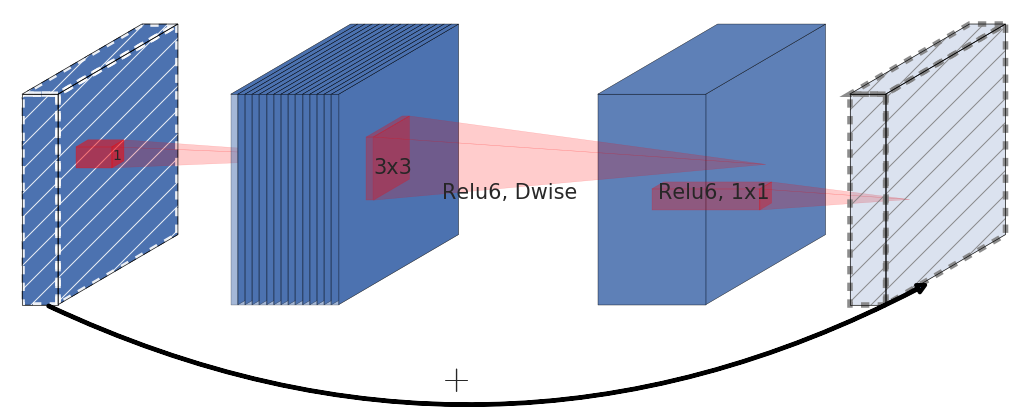
\includegraphics[width=0.4\textwidth]{residual_bottleneck}}
\caption{Bottleneck Schicht mit residualer Verbindung \cite{b5}}
\label{f1}
\end{figure}

MobileNet v2 besitzt mit diesem Aufbau insgesamt 3.47 Millionen Paramenter \cite{b4}.

Vergleicht man nun die Klassifikationsgenauigkeit von MobileNet v1 und MobileNet v2 auf dem ImageNet Datensatz erhält man folgende Werte:

\begin{table}[htbp]
\caption{Accuracy von MobileNet v1 und MobileNet v2 im Vergleich \cite{b4}}
\begin{center}
\begin{tabular}{|c|c|c|c|}
\hline
Architektur  & Anzahl Parameter & Top-1  & Top-5  \\
\hline
MobileNet v1 & 4.25 Millionen   & 70.9\% & 89.9\% \\
MobileNet v2 & 3.47 Millionen   & 71.8\% & 91.0\% \\
\hline
\end{tabular}
\end{center}
\end{table}

Man kann klar sehen, dass MobileNet v2 trotz verringerter Parameteranzahl eine bessere Genauigkeit auf dem ImageNet Datensatz aufweist.


\section{MobileNet v3 (2019)}
Während MobileNet v1 und MobileNet v2 Architekturen sind, die jeweils von Menschen erdacht und konzipiert wurden, wurde bei MobileNet v3 eine andere Strategie angewendet. Ein Forscherteam von Google AI und Google Brain hat für die MobileNet v3 Architektur das Neural Architecture Search (NAS) Verfahren angewendet und weitere manuelle Anpassungen vorgenommen. Von der MobileNet v3 Architektur gibt es 2 Varianten. Eine kleine (Small) und eine große Variante (Large).

\subsection{MobileNet v3 Large}
Als Grundlage für die große Variante wurde die durch Platform-Aware NAS entwickelte Architektur MnasNet-A1 gewählt \cite{b6}, welche ebenfalls wie MobileNet v2 Bottleneck Schichten verwendet. Diese Architektur wurde anschließend mittels des NetAdapt Algorithmus weiter optimiert und es wurden einige manuelle Anpassungen vorgenommen \cite{b6}. Zu diesen manuellen Anpassungen gehören zum einen, dass teure Schichten neu designt wurden, es wurde ReLU6 durch die Swish Aktivierungsfunktion ausgetauscht und es wurden squeeze-and-excitation (SE) Module eingebaut \cite{b4}.

Die SE Module sorgen dafür, dass das Netz lernt welche Channel wichtig sind und sich dann darauf konzentriert \cite{b4}. Dies wird dadurch erreicht, dass mittels Pooling die Eingabe der Größe $H \times W \times C$ auf eine Matrix der Größe $1 \times 1 \times C$ verkleinert wird (squeeze) und anschließend darauf eine Gewichtung angewendet wird (excitation). Der resultierende gewichtete Vektor wird dann mit der Eingabe multipliziert und man erhält einen eine Ausgabe der Größe $H \times W \times C$, bei der die einzelnen Channel unterschiedliche Gewichtungen haben.

Ein Bottleneck Block mit squeeze-and-excitation ist in \ref{f2} dargestellt.

\begin{figure}[htbp]
\centerline{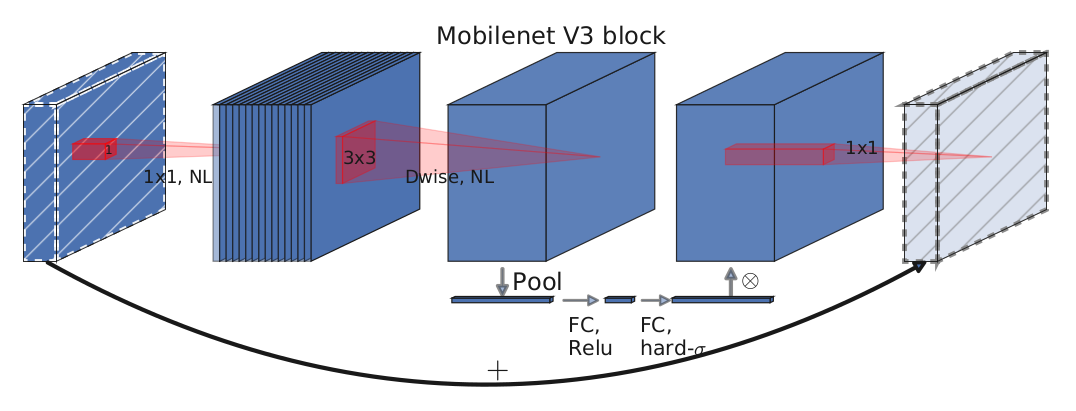
\includegraphics[width=0.4\textwidth]{squeeze_and_excitation}}
\caption{Bottleneck Schicht mit SE und residualer Verbindung \cite{b6}}
\label{f2}
\end{figure}

\subsection{MobileNet v3 Small}
Mit der kleinere Variante des MobileNet v3 sollte eine noch geringere Latenz erreicht werden als mit der größeren Variante. Aus diesem Grund wurde für die kleinere Variante eine neue Platform-Aware NAS Suche gestartet \cite{b6}.

Platform-Aware Neural Archtitecture Search ist eine Technik, bei der eine optimale Architektur für eine bestimmte Platform gesucht wird. Bei dem MobileNet v3 Small wurde dazu die Latenz der Architekturen auf real existierenden Mobilgeräten getestet und optimiert \cite{b6}. 

Nachdem eine grobe Architektur durch die NAS gefunden wurde, wurde diese erneut mittels NetAdapt Algorithmus optimiert. Anschließend wurden darauf noch die selben manuellen Anpassungen vorgenommen wie bei der großen Variante des MobileNet v3 \cite{b6}.

Auf dem ImageNet Datensatz \cite{b3} erreichen beide Architekturen folgende Genauigkeiten:

\begin{table}[htbp]
\caption{Accuracy von MobileNet v3 Small und Large im Vergleich \cite{b6}}
\begin{center}
\begin{tabular}{|c|c|c|c|}
\hline
Architektur        & Anzahl Parameter & Top-1 & Top-5  \\
\hline
MobileNet v3 Small & 2.9 Millionen   & 67.5\% & 87.7\% \\
MobileNet v3 Large & 5.4 Millionen   & 75.2\% & 92.2\% \\
\hline
\end{tabular}
\end{center}
\end{table}


\section{EfficientNet (2019, 2020)}
Wie bereits bei der MobileNet v1 Architektur gesehen, haben viele Architekturen eine Art Faktor mit der sich die Anzahl der Parameter und damit auch die Größe der Architektur verändern lässt. 
Generell kann die Größe der Architektur verändert werden, indem entweder die Breite (Anzahl der Channel in jedem Convolution Layer), die Tiefe (Anzahl der Schichten/Blöcke) oder die Auflösung des Eingabebildes verändert wird. Mit diesen drei Möglichkeiten kann die Anzahl der Parameter beeinflusst werden \cite{b7}.
Bei der MobileNet v1 Architektur wurde mittels des Depth Multipliers z.B. die Anzahl der Channels in den Convolution Layers verändert \cite{b4}.

\subsection{Compound Scaling}
Die Idee bei EfficientNet Architektur ist nun, dass ausgehend von einer Basisarchitektur (EfficientNet-B0) nun sowohl die Tiefe, Breite und die Auflösung gleichermaßen um einen bestimmten Faktor erhöht wird. Diese Methode wird in dem Paper Compound Scaling (Zusammengesetzte Skalierung) genannt\cite{b7}. Beim Compound Scaling wird ein Compound Koeffizient $\Phi$ und durch Grid-Search gefundene Konstanten $\alpha$, $\beta$, $\gamma$ mit $\alpha \geq 1 \land \beta \geq 1 \land \gamma \geq 1$ verwendet. Mittels folgender Regeln werden die Tiefe, Breite und Auflösung der abgeleiteten Architekturen für verschiedene $\Phi$ bestimmt \cite{b7}:
\begin{itemize}
\item Tiefe: $d = \alpha ^ \Phi$
\item Breite: $w = \beta ^ \Phi$
\item Auflösung: $r = \gamma ^ \Phi$
\end{itemize}

\subsection{EfficientNet-B0}
Die Basisarchitektur EfficientNet-B0 hat einen Compound Koeffizienten $\Phi = 1$ und wurde initial mittels Neural Architecture Search (NAS) gefunden. Diese Architektur ähnelt stark der MnasNet Architektur, welche ja auch schon als Grundlage für die MobileNet v3 Architektur gewählt wurde \cite{b4}. Dies liegt daran, da für diese Architektur der selbe Suchraum für den NAS Algorithmus verwendet wurde wie bei der MnasNet Architektur \cite{b7}. Es werden wie bei der MnasNet und MobileNet v3 Architektur Bottleneck Schichten, Depthwise Convolutions, squeeze-and-excitation Module und die Swish Aktivierungsfunktion verwendet \cite{b4}.

\subsection{Abgeleitete Architekturen}
Auf Basis der EfficientNet-B0 Architektur werden nun mittels Compound Scaling weitere Architekturen mit aufsteigend mehr Parametern abgeleitet. Insgesamt gibt es 8 Architekturen (B0 bis B7), welche mit verschiedenen Werten für $\Phi$ ermittelt wurden.

Auf dem ImageNet Datensatz \cite{b3} erreichen diese Architekturen folgende Genauigkeiten:

\begin{table}[htbp]
\caption{Accuracy der verschiedenen EfficientNet Architekturen \cite{b7}}
\begin{center}
\begin{tabular}{|c|c|c|c|}
\hline
Architektur     & Anzahl Parameter & Top-1  & Top-5  \\
\hline
EfficientNet-B0 & 5.3 Millionen    & 77.1\% & 93.3\% \\
EfficientNet-B1 & 7.8 Millionen    & 79.1\% & 94.4\% \\
EfficientNet-B2 & 9.2 Millionen    & 80.1\% & 94.9\% \\
EfficientNet-B3 & 12 Millionen     & 81.6\% & 95.7\% \\
EfficientNet-B4 & 19 Millionen     & 82.9\% & 96.4\% \\
EfficientNet-B5 & 30 Millionen     & 83.6\% & 96.7\% \\
EfficientNet-B6 & 43 Millionen     & 84.0\% & 96.8\% \\
EfficientNet-B7 & 66 Millionen     & 84.3\% & 97.0\% \\
\hline
\end{tabular}
\end{center}
\end{table}

\subsection{EfficientNet Lite}
Zusätzlich zu den normalen EfficientNet Architekturen wurden im Jahr 2020 fünf neue Architekturen veröffentlicht (lite0 bis lite4).
Bei diesen Architekturen wurden folgende Änderungen vorgenommen. Zum einen wurde squeeze-and-excitation entfernt, da diese Operation auf einiger Hardware nicht unterstützt ist. Zusätzlich wurde die Swish Aktivierungsfunktion ausgetauscht um eine besser Quantisierbarkeit der Modelle zu gewährleisten
Außerdem wurden einige Parameter beim Compound Scaling ausgeschlossen, da dadurch die Größe und Anzahl an Berechnungen verringert wird \cite{b8}.

Schaut man sich die Genauigkeit auf den ImageNet Daten \cite{b3} an ergibt sich folgendes:

\begin{table}[htbp]
\caption{Accuracy der EfficientNet Lite Architekturen \cite{b4}}
\begin{center}
\begin{tabular}{|c|c|c|c|}
\hline
Architektur     & Anzahl Parameter & Top-1  & Top-5  \\
\hline
EfficientNet-lite0 & 4.7 Millionen    & 74.8\% & 92.2\% \\
EfficientNet-lite1 & 5.4 Millionen    & 76.6\% & 93.2\% \\
EfficientNet-lite2 & 6.1 Millionen    & 77.5\% & 93.7\% \\
EfficientNet-lite3 & 8.2 Millionen    & 79.8\% & 94.9\% \\
EfficientNet-lite4 & 13 Millionen     & 81.5\% & 95.7\% \\
\hline
\end{tabular}
\end{center}
\end{table}


\section{Anwendungsmöglichkeiten und Nutzbarkeit}

\subsection{Anwendungsmöglichkeiten}
Die vorgestellten Architekturen haben alle das Ziel möglichst effizient gute Ergebnisse zu erreichen. Aus diesem Grund eignen sich diese Architekturen besonders gut für den Einsatz in eingebetteten und mobilen Anwendungsbereichen wo es oft an Rechen- und Speicherkapazität fehlt.

Anwendungen für diese Architekturen sind vorrangig Klassifikationsprobleme auf Bilddaten wie zum Beispiel die Klassifikation von Bildern, wie es beim ImageNet Datensatz gemacht wird \cite{b3}.
Möglich ist z.B. die Klassifikation von Fahrzeugen beim autonomen Fahren oder die Diagnose von Malaria mittels Blutabstrichen.
Aber auch Geolokalisierung ist möglich, wenn dieses Problem als Klassifikationsproblem auffasst wird, indem die Erde in ein Gitter von Zellen aufteilt wird und dann das Netz mit Bildern aus diesen Gitterzellen trainiert wird \cite{b9}. Ein weiteres Klassifikationsproblem, was mittels diesen Architekturen möglich ist, ist das Ermitteln von Gesichtseigenschaften \cite{b9}.

Aber zusätzlich lassen sich diese Architekturen auch als Feature Extractor nutzen was eine Vielzahl weiterer Anwendungsmöglichkeiten eröffnet. Zum Beispiel können diese Architekturen auch als Teil einer Architektur für die Objekterkennung eingesetzt werden \cite{b9}.

\subsection{Nutzbarkeit}
Neben der Vielzahl an Anwendungsmöglichkeiten dieser Architekturen muss aber auch die Verwendbarkeit und Verfügbarkeit in Betracht gezogen werden.
Mit Verfügbarkeit ist in diesem Paper das Vorhandensein von nutzbaren Implementationen in der Python-Bibliothek TensorFlow 2.
Dazu werden die vorgestellten Architekturen im folgenden kurz besprochen.

\subsubsection{SqueezeNet}
SqueezeNet ist die älteste der vorgestellten Architekturen. Für diese Architektur gibt es keine nutzbare TensorFlow 2 Implementation. Die einzigen Implementationen welche sich finden sind TensorFlow 1 Implementationen. Jedoch gibt es für diese Architektur eine Implementation in PyTorch. Generell muss aber auch die Genauigkeit von SqueezeNet betrachtet werden, welche heute nicht mehr dem Stand der Technik entspricht und es ratsam ist stattdessen MobileNets oder EfficientNets zu verwenden. Trotzdem ist diese Architektur die kleinste der vorgestellten Architekturen.

\subsubsection{MobileNet}
Die MobileNet Architekturen sind sehr verbreitet und werden in allen Varianten von TensorFlow 2 unterstützt. Das bedeutet es gibt in dem tf.keras.applications Modul Implementationen für das MobileNet v1, MobileNet v2, MobileNet v3 small und MobileNet v3 large. Zusätzlich dazu können diese Architekturen sowohl vortrainiert auf den ImageNet Datensatz verwendet werden, als auch von Grund auf neu trainiert werden.

\subsubsection{EfficientNet}
Die normalen EfficientNet Architekturen (B0 - B7) sind von TensorFlow 2 ebenfalls im Modul tf.keras.applications vollständig vorhanden und können genauso wie bei den MobileNets auch, sowohl vortrainiert auf den ImageNet Daten als auch nicht vortrainiert verwendet werden. Jedoch gilt bei der Verwendbarkeit von den EfficientNet Architekturen im eingebetteten und mobilen Szenario zu beachten, dass ab EfficientNet-B2, welches schon 9.2 Millionen Parameter besitzt, die Architekturen immer größer werden und nur noch begrenzt bis gar nicht in dem Anwendungsfeld einsetzbar sind. Das heißt für eingebettet und mobile Systeme sind hauptsächlich die EfficientNet-B0 bis EfficientNet-B2 relevant.

\subsubsection{EfficientNet Lite}
Die EfficientNet Lite Architekturen sind relativ neu erschienen (2020). Aus diesem Grund sind sie bisher noch nicht so gut in TensorFlow 2 implementiert. Es gibt im TensorFlow Hub vortrainierte TensorFlow 1 Modelle für diese Architektur, dessen Kompatibilität mit TensorFlow 2 jedoch eingeschränkt ist und es gibt für PyTorch eine Implementation dieser Architektur. Des Weiteren fehlen zu den EfficientNet Lite Architekturen genauere Beschreibungen in Form eines Papers. Es gibt lediglich einen Blogeintrag von TensorFlow \cite{b8}, welcher die Änderungen der EfficientNet Lite Architekturen zu den normalen EfficientNet Architekturen beschreibt. Damit ist diese Architektur sehr eingeschränkt nutzbar.


\begin{thebibliography}{00}
\bibitem{b1} F. N. Iandola, S. Han, M. W. Moskewicz, K. Ashraf, W. J. Dally, K. Keutzer. (2016). SqueezeNet: AlexNet-level accuracy with 50x fewer parameters and $<$0.5MB model size.

\bibitem{b2} A. Krizhevsky, I. Sutskever, and G. E. Hinton. ImageNet Classification with Deep Convolutional Neural Networks. In NIPS, 2012.

\bibitem{b3} Olga Russakovsky*, Jia Deng*, Hao Su, Jonathan Krause, Sanjeev Satheesh, Sean Ma, Zhiheng Huang, Andrej Karpathy, Aditya Khosla, Michael Bernstein, Alexander C. Berg and Li Fei-Fei. (* = equal contribution) ImageNet Large Scale Visual Recognition Challenge. IJCV, 2015.

\bibitem{b4} Hollemans, M., 2020. New Mobile Neural Network Architectures. [online] Machinethink.net. Available at: https://machinethink.net/blog/mobile-architectures/ [Accessed 6 November 2020].

\bibitem{b5} M. Sandler, A. Howard, M. Zhu, A. Zhmoginov and L. Chen, "MobileNetV2: Inverted Residuals and Linear Bottlenecks," 2018 IEEE/CVF Conference on Computer Vision and Pattern Recognition, Salt Lake City, UT, 2018, pp. 4510-4520, doi: 10.1109/CVPR.2018.00474.

\bibitem{b6} A. Howard et al., "Searching for MobileNetV3," 2019 IEEE/CVF International Conference on Computer Vision (ICCV), Seoul, Korea (South), 2019, pp. 1314-1324, doi: 10.1109/ICCV.2019.00140.

\bibitem{b7} Tan, Mingxing, and Quoc V. Le. "Efficientnet: Rethinking model scaling for convolutional neural networks." arXiv preprint arXiv:1905.11946 (2019).

\bibitem{b8} R. Liu, "Higher accuracy on vision models with EfficientNet-Lite" TensorFlow Blog, Mar. 16, 2020. https://blog.tensorflow.org/2020/03/higher-accuracy-on-vision-models-with-efficientnet-lite.html.

\bibitem{b9} A. G. Howard et al., “MobileNets: Efficient Convolutional Neural Networks for Mobile Vision Applications,” arXiv.org, 2017. https://arxiv.org/abs/1704.04861.
\end{thebibliography}

\end{document}
